\documentclass[11pt,psfig]{article}
\usepackage{epsfig}
\usepackage{times}
\usepackage{amssymb}
\usepackage{float}

\newcount\refno\refno=1
\def\ref{\the\refno \global\advance\refno by 1}
\def\ux{\underline{x}}
\def\uw{\underline{w}}
\def\bw{\underline{w}}
\def\ut{\underline{\theta}}
\def\umu{\underline{\mu}} 
\def\bmu{\underline{\mu}} 
\def\be{p_e^*}
\newcount\eqnumber\eqnumber=1
\def\eq{\the \eqnumber \global\advance\eqnumber by 1}
\def\eqs{\eq}
\def\eqn{\eqno(\eq)}

 \pagestyle{empty}
\def\baselinestretch{1.1}
\topmargin1in \headsep0.3in
\topmargin0in \oddsidemargin0in \textwidth6.5in \textheight8.5in
\begin{document}
\setlength{\parskip}{1.2ex plus0.3ex minus 0.3ex}


\thispagestyle{empty} \pagestyle{myheadings} \markright{Homework
3: CS 216, Image Understanding: Spring 2014}



\title{CS 216 Homework 3}
\author{Zachary DeStefano, 15247592}
\date{Due Date: May 9, 2014 in class}

\maketitle

\vfill\eject

\newpage

\section*{Problem 1}

\subsection*{k-Means Clustering results}

\begin{figure}[H]
\centering
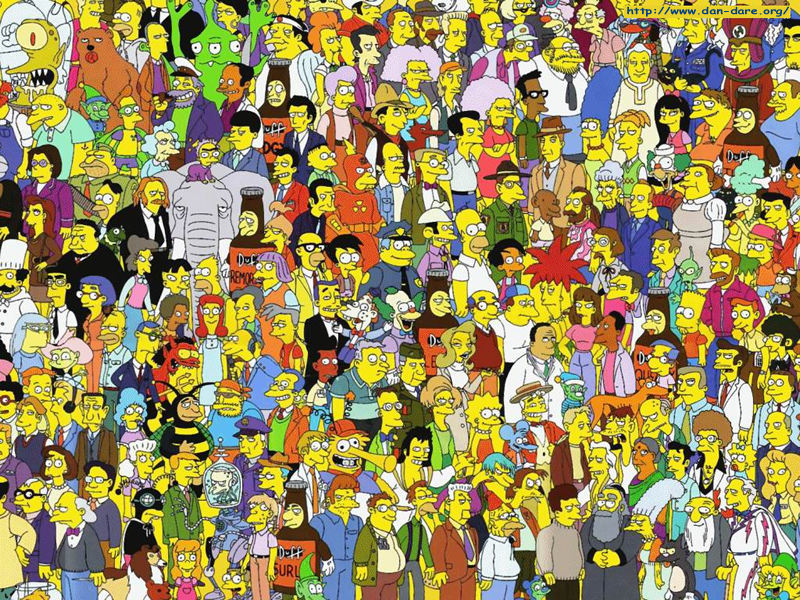
\includegraphics[height=3in]{simpsons.jpg}
\caption{Original Image}
\end{figure}

\begin{figure}[H]
\centering
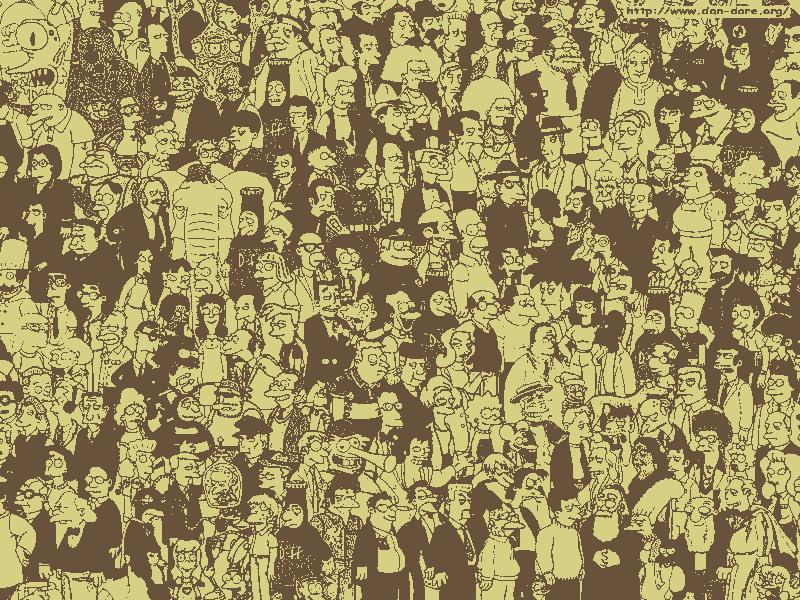
\includegraphics[height=3in]{2-means_simpsons.jpg}
\caption{The k-Means Image when $k=2$}
\end{figure}

\begin{figure}[H]
\centering
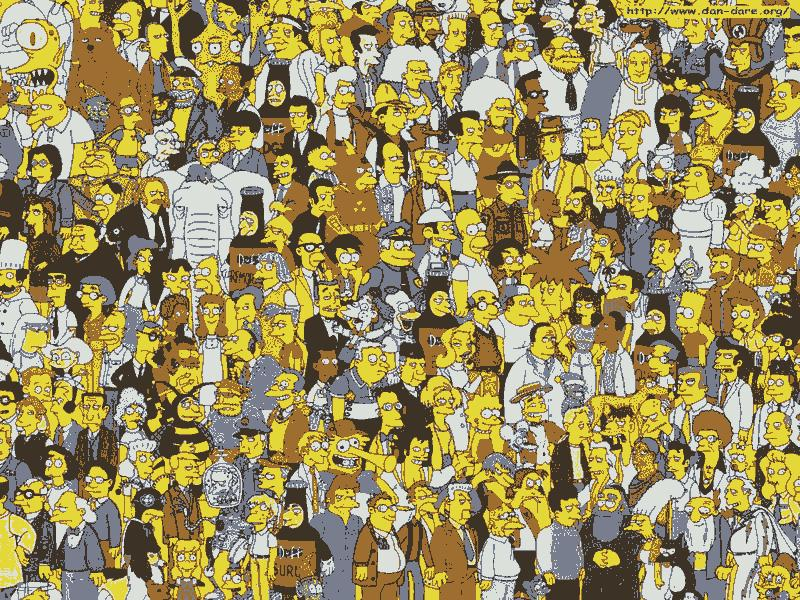
\includegraphics[height=3in]{5-means_simpsons.jpg}
\caption{The k-Means Image when $k=5$}
\end{figure}

\begin{figure}[H]
\centering
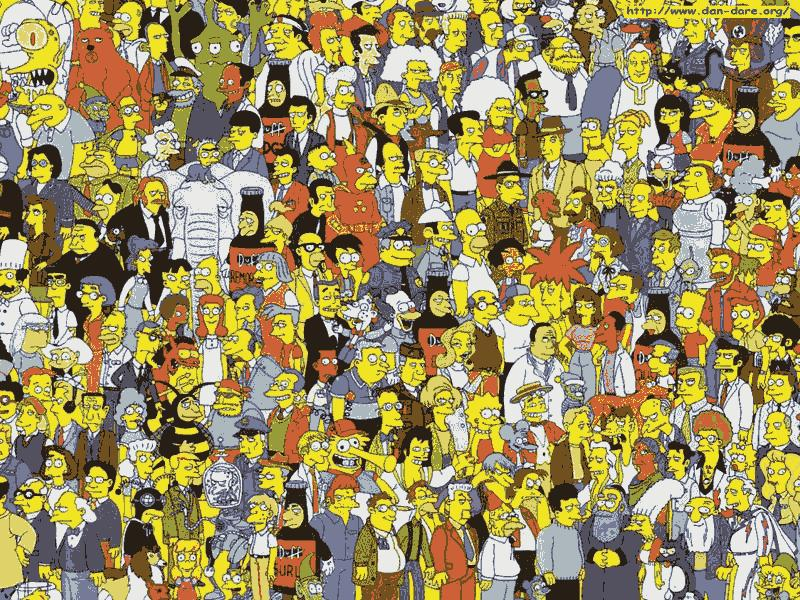
\includegraphics[height=3in]{10-means_simpsons.jpg}
\caption{The k-Means Image when $k=10$}
\end{figure}

\subsection*{Result when skewing the Red Channel}

If we multiply the red channel by 100, then the mean will tend more toward the red channel than the other channels. The result will be a red tint on the final result image. That is exactly what happened with the following images which are the same k-means images as above but the red channel was multiplied by 100 before k-Means was done. 

\begin{figure}[H]
\centering
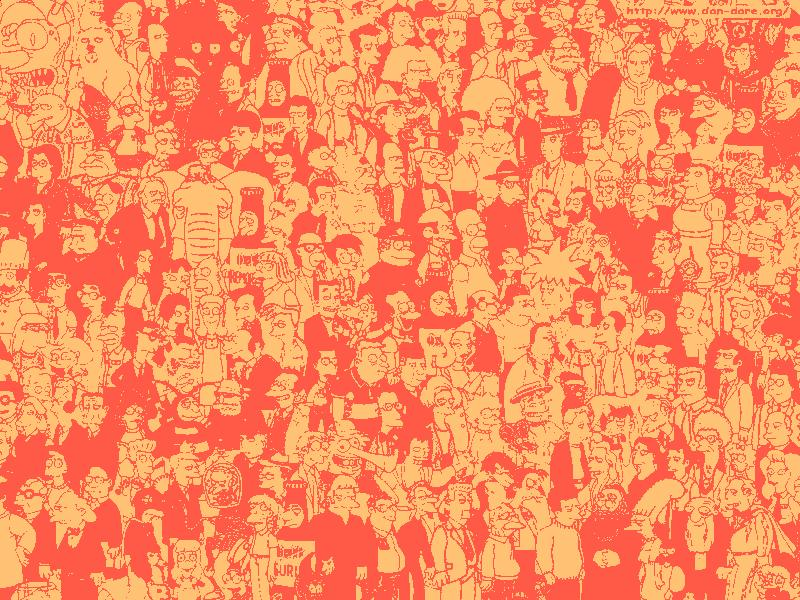
\includegraphics[height=3in]{2-means_redEn_simpsons.jpg}
\caption{The k-Means Image when $k=2$ and a skewed red channel}
\end{figure}

\begin{figure}[H]
\centering
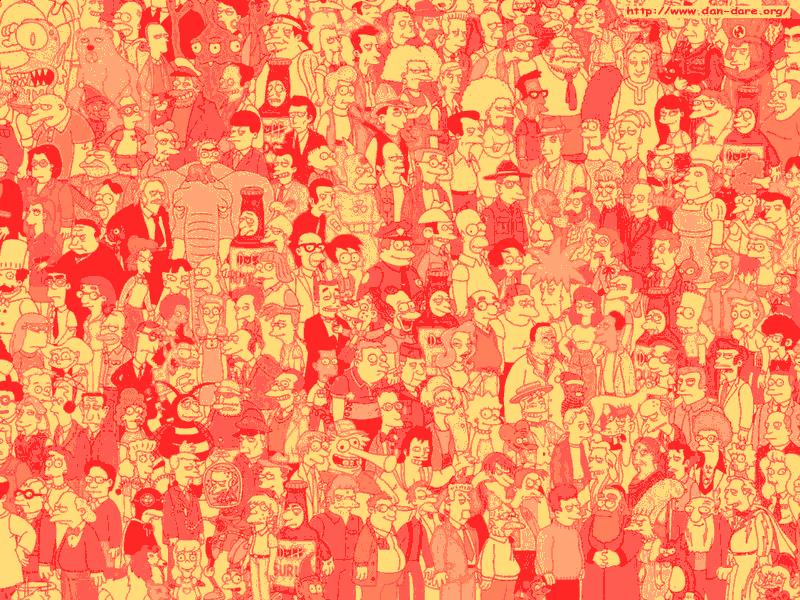
\includegraphics[height=3in]{5-means_redEn_simpsons.jpg}
\caption{The k-Means Image when $k=5$ and a skewed red channel}
\end{figure}

\begin{figure}[H]
\centering
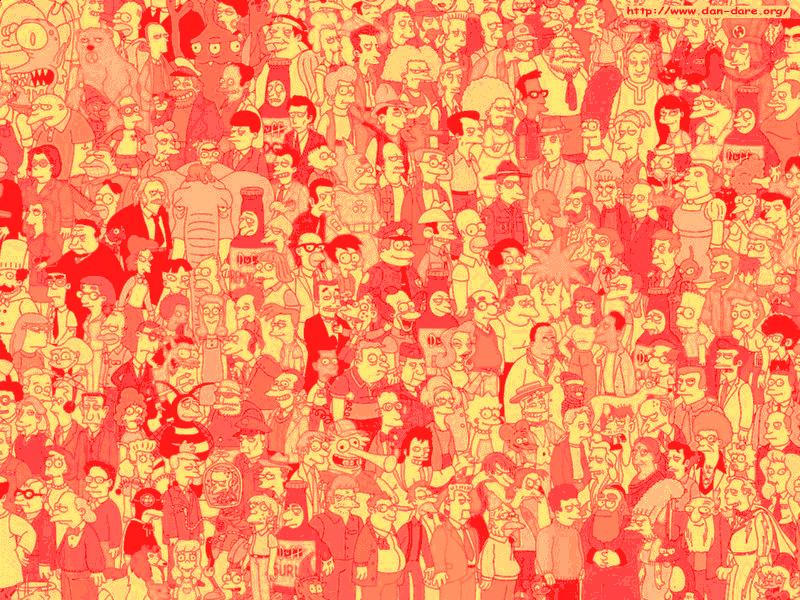
\includegraphics[height=3in]{10-means_redEn_simpsons.jpg}
\caption{The k-Means Image when $k=10$ and a skewed red channel}
\end{figure}

\newpage

\section*{Problem 2}

Here is my original image:

\begin{figure}[H]
\centering
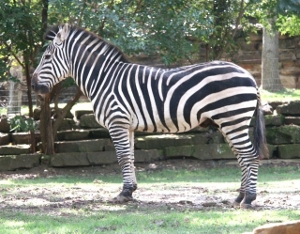
\includegraphics[height=3in]{zebra_small.jpg}
\caption{The image of the zebra}
\end{figure}

\subsection*{8 filter images}

\begin{figure}[H]
\centering
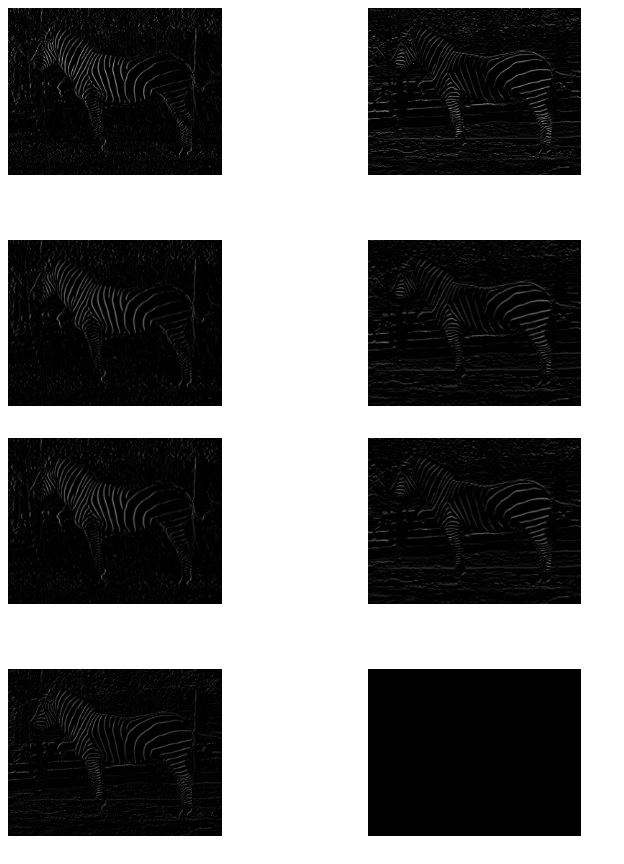
\includegraphics[width=7in]{prob2filterImages.jpg}
\caption{The Filter Images}
\end{figure}

\subsection*{Matlab code}

Here is the parent script that calls the function:

\begin{verbatim}


imname = 'zebra_small.jpg';
imageData = im2double(rgb2gray(imread(imname)));
%
%h1 means horizontal derivative, sigma 1
%h2, h4, v1, v2, v4 follow the same thing
%g42 is gaussian 4-2, g21 is similar
[h1,v1,h2,v2,h4,v4,g42,g21] = get8FilterImages(imageData);
figure

subplot(2,4,1)
imshow(h1,[])
title('Horiz,sigma=1');

subplot(2,4,2)
imshow(h2,[])
title('Horiz,sigma=2');

subplot(2,4,3)
imshow(h4,[])
title('Horiz,sigma=4');

subplot(2,4,4)
imshow(g42,[])
title('G_4 - G_2');

subplot(2,4,5)
imshow(v1,[])
title('Vert,sigma=1');

subplot(2,4,6)
imshow(v2,[])
title('Vert,sigma=2');

subplot(2,4,7)
imshow(v4,[])
title('Vert,sigma=4');

subplot(2,4,8)
imshow(g21,[])
title('G_2-G_1');
\end{verbatim}

Here is the main function that gets the information:

\begin{verbatim}

function [ horizDeriv_Sigma1_imageData,vertDeriv_Sigma1_imageData,...
    horizDeriv_Sigma2_imageData,vertDeriv_Sigma2_imageData,...
    horizDeriv_Sigma4_imageData,vertDeriv_Sigma4_imageData,...
    gaussDiff_4_2_imageData,gaussDiff_2_1_imageData] = get8FilterImages( imageData )
%GET8FILTERIMAGES Summary of this function goes here
%   Detailed explanation goes here

[horizDeriv_Sigma1_imageData,vertDeriv_Sigma1_imageData] =...
    computeDerivImages(imageData,1);
[horizDeriv_Sigma2_imageData,vertDeriv_Sigma2_imageData] =...
    computeDerivImages(imageData,2);
[horizDeriv_Sigma4_imageData,vertDeriv_Sigma4_imageData] =...
    computeDerivImages(imageData,4);
gaussDiff_4_2_imageData = computeGaussDiff(imageData,1,2);
gaussDiff_2_1_imageData = computeGaussDiff(imageData,2,4);
end

\end{verbatim}

This is the helper function that gets the gaussian derivatives:

\begin{verbatim}
function [horizDerivImage,vertDerivImage] = computeDerivImages( imageData,sigma )
%COMPUTEDERIVIMAGES Summary of this function goes here
%   Detailed explanation goes here

gaussFilt = fspecial('gaussian',sigma);
rowNum = ceil(sigma/2);
gaussFilter = gaussFilt(rowNum,:);
filteredImageData = conv2(imageData,gaussFilter,'same');
horizDerivFilter = [1 -1];
horizDerivImage = conv2(filteredImageData,horizDerivFilter,'same');
vertDerivFilter = [1;-1];
vertDerivImage = conv2(filteredImageData,vertDerivFilter,'same');

end
\end{verbatim}

This is the helper function that computes the gaussian differences

\begin{verbatim}
function [filterDiffImageData] = computeGaussDiff( imageData,sigma1,sigma2 )
%COMPUTEDERIVIMAGES Summary of this function goes here
%   Detailed explanation goes here

gaussFilt1 = fspecial('gaussian',sigma1);
gaussFilt2 = fspecial('gaussian',sigma2);
filteredImageData1 = conv2(imageData,gaussFilt1,'same');
filteredImageData2 = conv2(imageData,gaussFilt2,'same');
filterDiffImageData = filteredImageData2-filteredImageData1;

end
\end{verbatim}

\newpage

\section*{Problem 3}

These are the image patches that were filtered and then analyzed. The left one is the neck of the zebra. The middle one is the picture of the tree leaves above the zebra's back. The right one is the grass in front of the zebra. The radius of the patch was scaled and it was scaled in such a way so that the patch would capture that object and only that object. 

\begin{figure}[H]
\centering
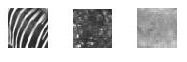
\includegraphics[width=3in]{prob3patches.jpg}
\caption{Image Patches that were analyzed}
\end{figure}

Here is the visualization for each of the mean absolute response vectors. 

\begin{figure}[H]
\centering
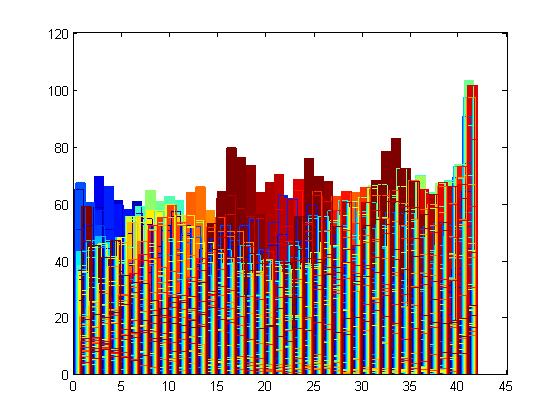
\includegraphics[height=3in]{prob3patch1bar.jpg}
\caption{Bar graph visualization for the neck image patch}
\end{figure}

\begin{figure}[H]
\centering
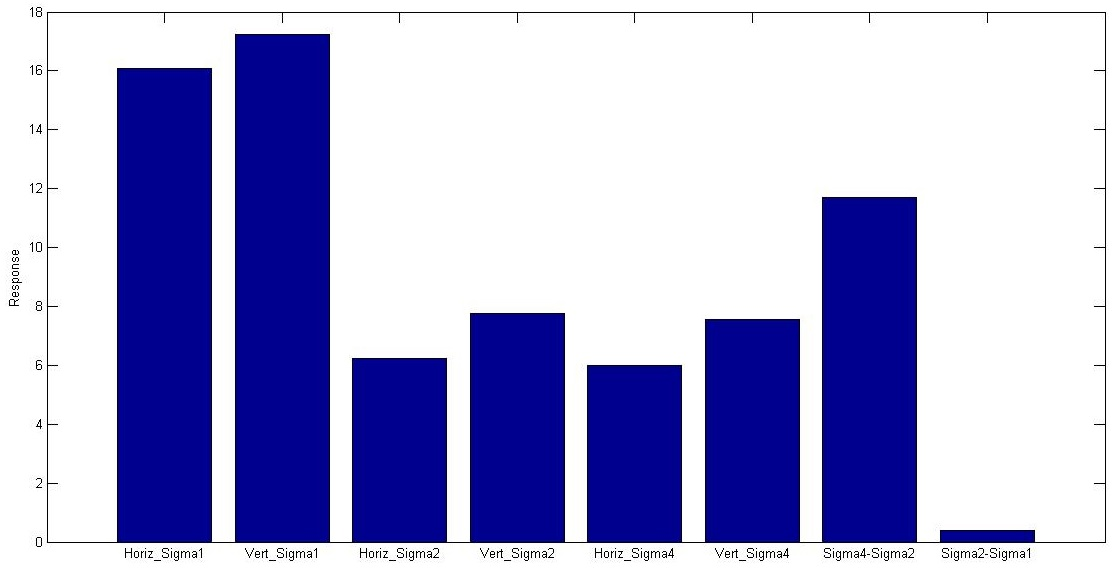
\includegraphics[height=3in]{prob3patch2bar.jpg}
\caption{Bar graph visualization for the leaves image patch}
\end{figure}

\begin{figure}[H]
\centering
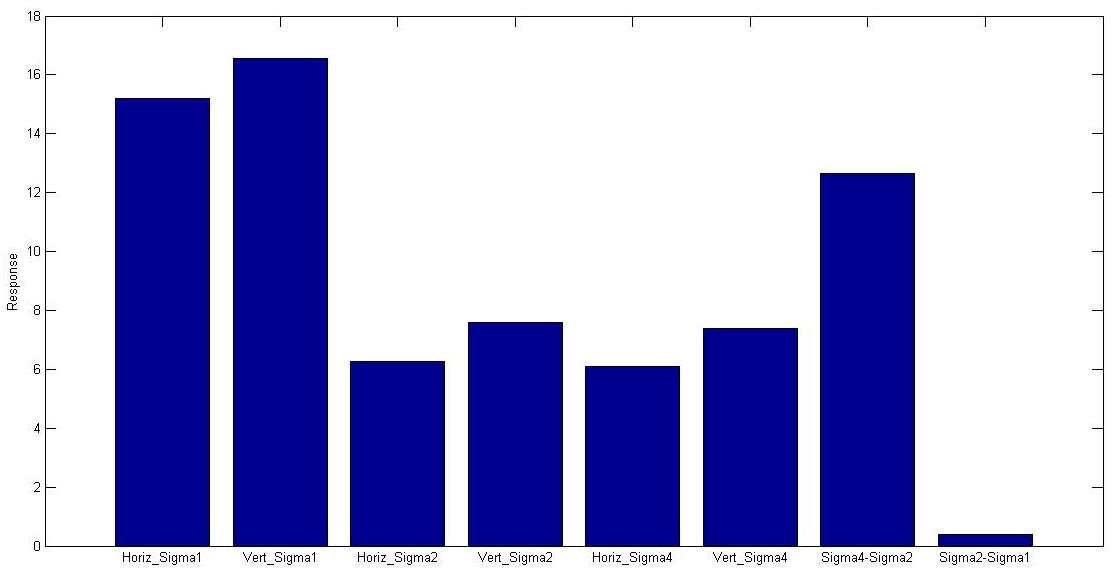
\includegraphics[height=3in]{prob3patch3bar.jpg}
\caption{Bar graph visualization for the grass image patch}
\end{figure}

Here are the filterbank images for each of those patches. 

\begin{figure}[H]
\centering
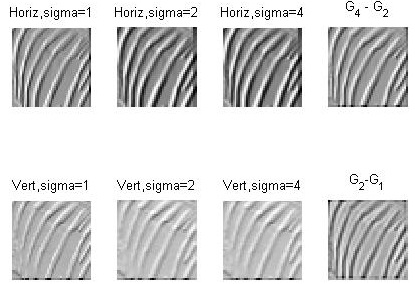
\includegraphics[height=2in]{prob3patch1filter.jpg}
\caption{Filterbank for the neck image patch}
\end{figure}

\begin{figure}[H]
\centering
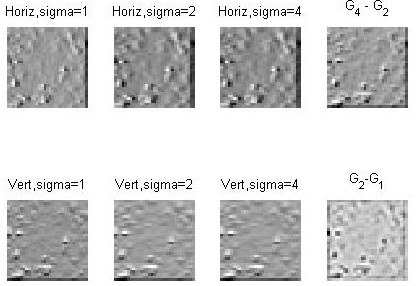
\includegraphics[height=2in]{prob3patch2filter.jpg}
\caption{Filterbank for the leaves image patch}
\end{figure}

\begin{figure}[H]
\centering
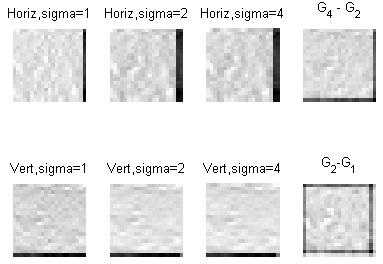
\includegraphics[height=2in]{prob3patch3filter.jpg}
\caption{Filterbank for the grass image patch}
\end{figure}

\newpage

\section*{Problem 4}

Here is the color map created by applying the 8 filters to the zebra picture above and then running k-means on the 8-dimensional data created by putting all the images into one large array. 

\begin{figure}[H]
\centering
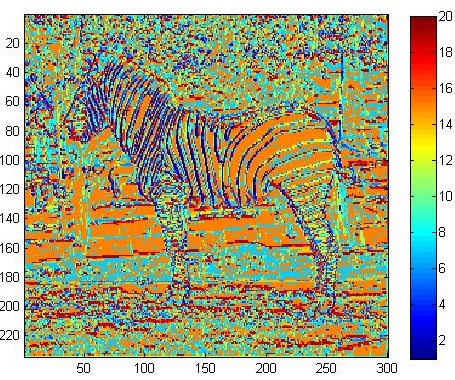
\includegraphics[height=4in]{prob4plot.jpg}
\caption{Imagesc visualization of the cluster center labels for the zebra image}
\end{figure}

\newpage

\section*{Problem 5}

\subsection*{Part A}

For segtest2.jpg, the results were really nice. The dragon ended up in the foreground and the rest of the image was in the background as expected. There did not need to be any tuning of the $\lambda$ to accomplish that. Here is the result:

\begin{figure}[H]
\centering
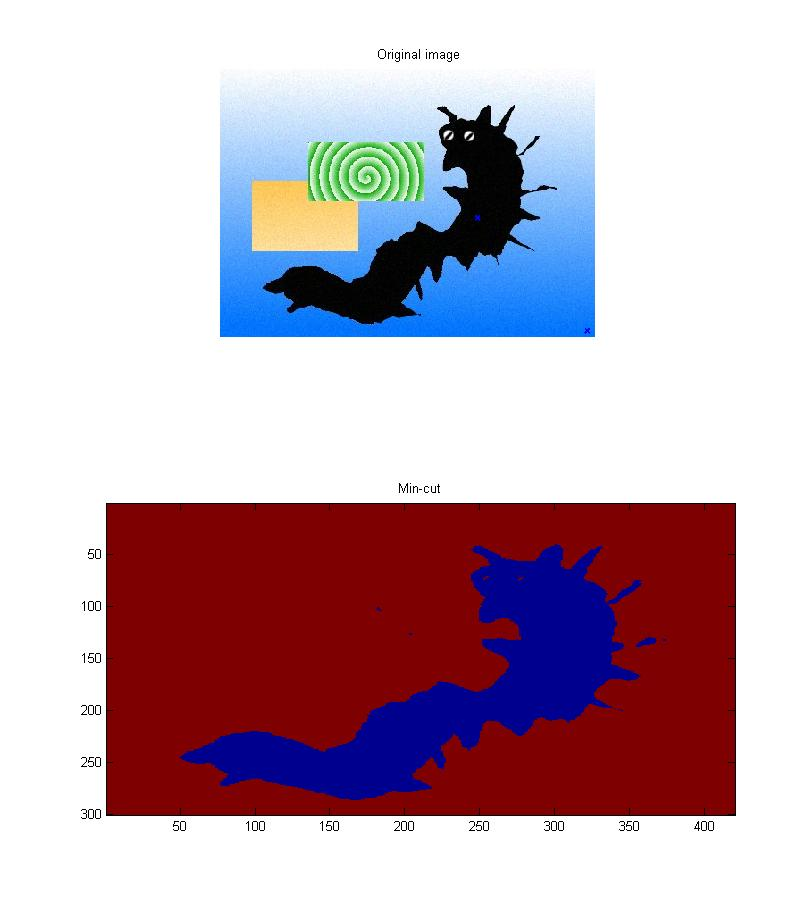
\includegraphics[width=4in]{prob5plotA.jpg}
\caption{Min cut results for segtest2.jpg}
\end{figure}

For segtest1.jpg, the results were worse. I tried to make the maroon ball the foreground and the rest the background but it did not quite divide it that way.

\begin{figure}[H]
\centering
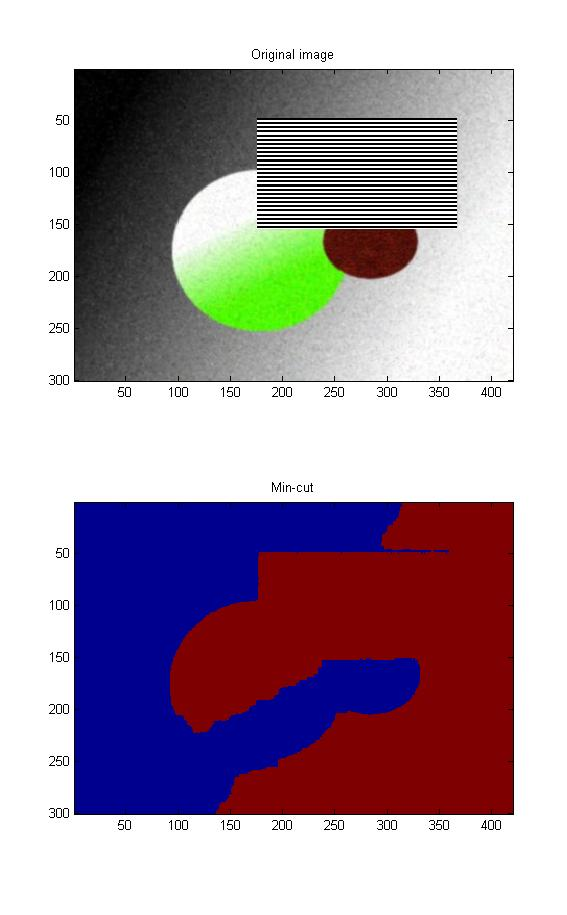
\includegraphics[width=4in]{prob5plotA_2.jpg}
\caption{Min cut results for segtest1.jpg}
\end{figure}

\newpage

\section*{Problem 6}

In the Department of Ophthalmology at UC Irvine, they have pictures of collagen fibers in the eye and they want to use these pictures as a basis for a 3D reconstruction of the fibers. The first step in the 3D reconstruction will be segmenting the images and putting them together. In the images, the fibers look like lines stacked up on top of each other. These lines can merge together as well as split apart into two lines. \\
\\
Here is a rough outline of the steps of the project: \\
1. Segment the images to extract out the line data. \\
2. Use the line information to line up images side by side \\
3. Get long images that are formed by a series of images put side by side \\

\end{document}








